\documentclass[11pt, a4paper]{article}
\usepackage{pdfpages}
\usepackage{parallel}
\usepackage[T2A]{fontenc}
\usepackage{ucs}
\usepackage[utf8x]{inputenc}
\usepackage[polish,english,russian]{babel}
\usepackage{hyperref}
\usepackage{rotating}
\usepackage[inner=2cm,top=1.8cm,outer=2cm,bottom=2.3cm,nohead]{geometry}
\usepackage{listings}
\usepackage{graphicx}
\usepackage{wrapfig}
\usepackage{longtable}
\usepackage{indentfirst}
\usepackage{array}
\usepackage{tikzsymbols}
\usepackage{soul}
\usepackage[ruled,vlined]{algorithm2e}
%\counterwithout{figure}{section} 

\usepackage{url}
\makeatletter
\g@addto@macro{\UrlBreaks}{\UrlOrds}
\makeatother

\newcolumntype{P}[1]{>{\raggedright\arraybackslash}p{#1}}
\frenchspacing
\usepackage{fixltx2e} %text sub- and superscripts
\usepackage{icomma} % коскі ў матэматычным рэжыме
\PreloadUnicodePage{4}

\newcommand{\longpage}{\enlargethispage{\baselineskip}}
\newcommand{\shortpage}{\enlargethispage{-\baselineskip}}

\def\switchlang#1{\expandafter\csname switchlang#1\endcsname}
\def\switchlangbe{
\let\saverefname=\refname%
\def\refname{Літаратура}%
\def\figurename{Іл.}%
}
\def\switchlangen{
\let\saverefname=\refname%
\def\refname{References}%
\def\figurename{Fig.}%
}
\def\switchlangru{
\let\saverefname=\refname%
\let\savefigurename=\figurename%
\def\refname{Литература}%
\def\figurename{Рис.}%
}

\hyphenation{admi-ni-stra-tive}
\hyphenation{ex-pe-ri-ence}
\hyphenation{fle-xi-bi-li-ty}
\hyphenation{Py-thon}
\hyphenation{ma-the-ma-ti-cal}
\hyphenation{re-ported}
\hyphenation{imp-le-menta-tions}
\hyphenation{pro-vides}
\hyphenation{en-gi-neering}
\hyphenation{com-pa-ti-bi-li-ty}
\hyphenation{im-pos-sible}
\hyphenation{desk-top}
\hyphenation{elec-tro-nic}
\hyphenation{com-pa-ny}
\hyphenation{de-ve-lop-ment}
\hyphenation{de-ve-loping}
\hyphenation{de-ve-lop}
\hyphenation{da-ta-ba-se}
\hyphenation{plat-forms}
\hyphenation{or-ga-ni-za-tion}
\hyphenation{pro-gramming}
\hyphenation{in-stru-ments}
\hyphenation{Li-nux}
\hyphenation{sour-ce}
\hyphenation{en-vi-ron-ment}
\hyphenation{Te-le-pathy}
\hyphenation{Li-nux-ov-ka}
\hyphenation{Open-BSD}
\hyphenation{Free-BSD}
\hyphenation{men-ti-on-ed}
\hyphenation{app-li-ca-tion}

\def\progref!#1!{\texttt{#1}}
\renewcommand{\arraystretch}{2} %Іначай формулы ў матрыцы зліпаюцца з лініямі
\usepackage{array}

\def\interview #1 (#2), #3, #4, #5\par{

\section[#1, #3, #4]{#1 -- #3, #4}
\def\qname{LVEE}
\def\aname{#1}
\def\q ##1\par{{\noindent \bf \qname: ##1 }\par}
\def\a{{\noindent \bf \aname: } \def\qname{L}\def\aname{#2}}
}

\def\interview* #1 (#2), #3, #4, #5\par{

\section*{#1\\{\small\rm #3, #4. #5}}
\ifx\ParallelWhichBox\undefined%
    \addcontentsline{toc}{section}{#1, #3, #4}%
\else%
\ifnum\ParallelWhichBox=0%
    \addcontentsline{toc}{section}{#1, #3, #4}%
\fi\fi%

\def\qname{LVEE}
\def\aname{#1}
\def\q ##1\par{{\noindent \bf \qname: ##1 }\par}
\def\a{{\noindent \bf \aname: } \def\qname{L}\def\aname{#2}}
}

\newcommand{\interviewfooter}[1]{
\vskip 1em
\noindent \textit{#1}
}


\begin{document}

\title{1992 "--- Lotus Mouse}
\date{}
\maketitle

Lotus Mouse является характерным примером оптомеханического манипулятора 90-х годов. Внешний вид данной мыши можно видеть на рис. \ref{fig:LotusPic}.

\begin{figure}[h]
    \centering
    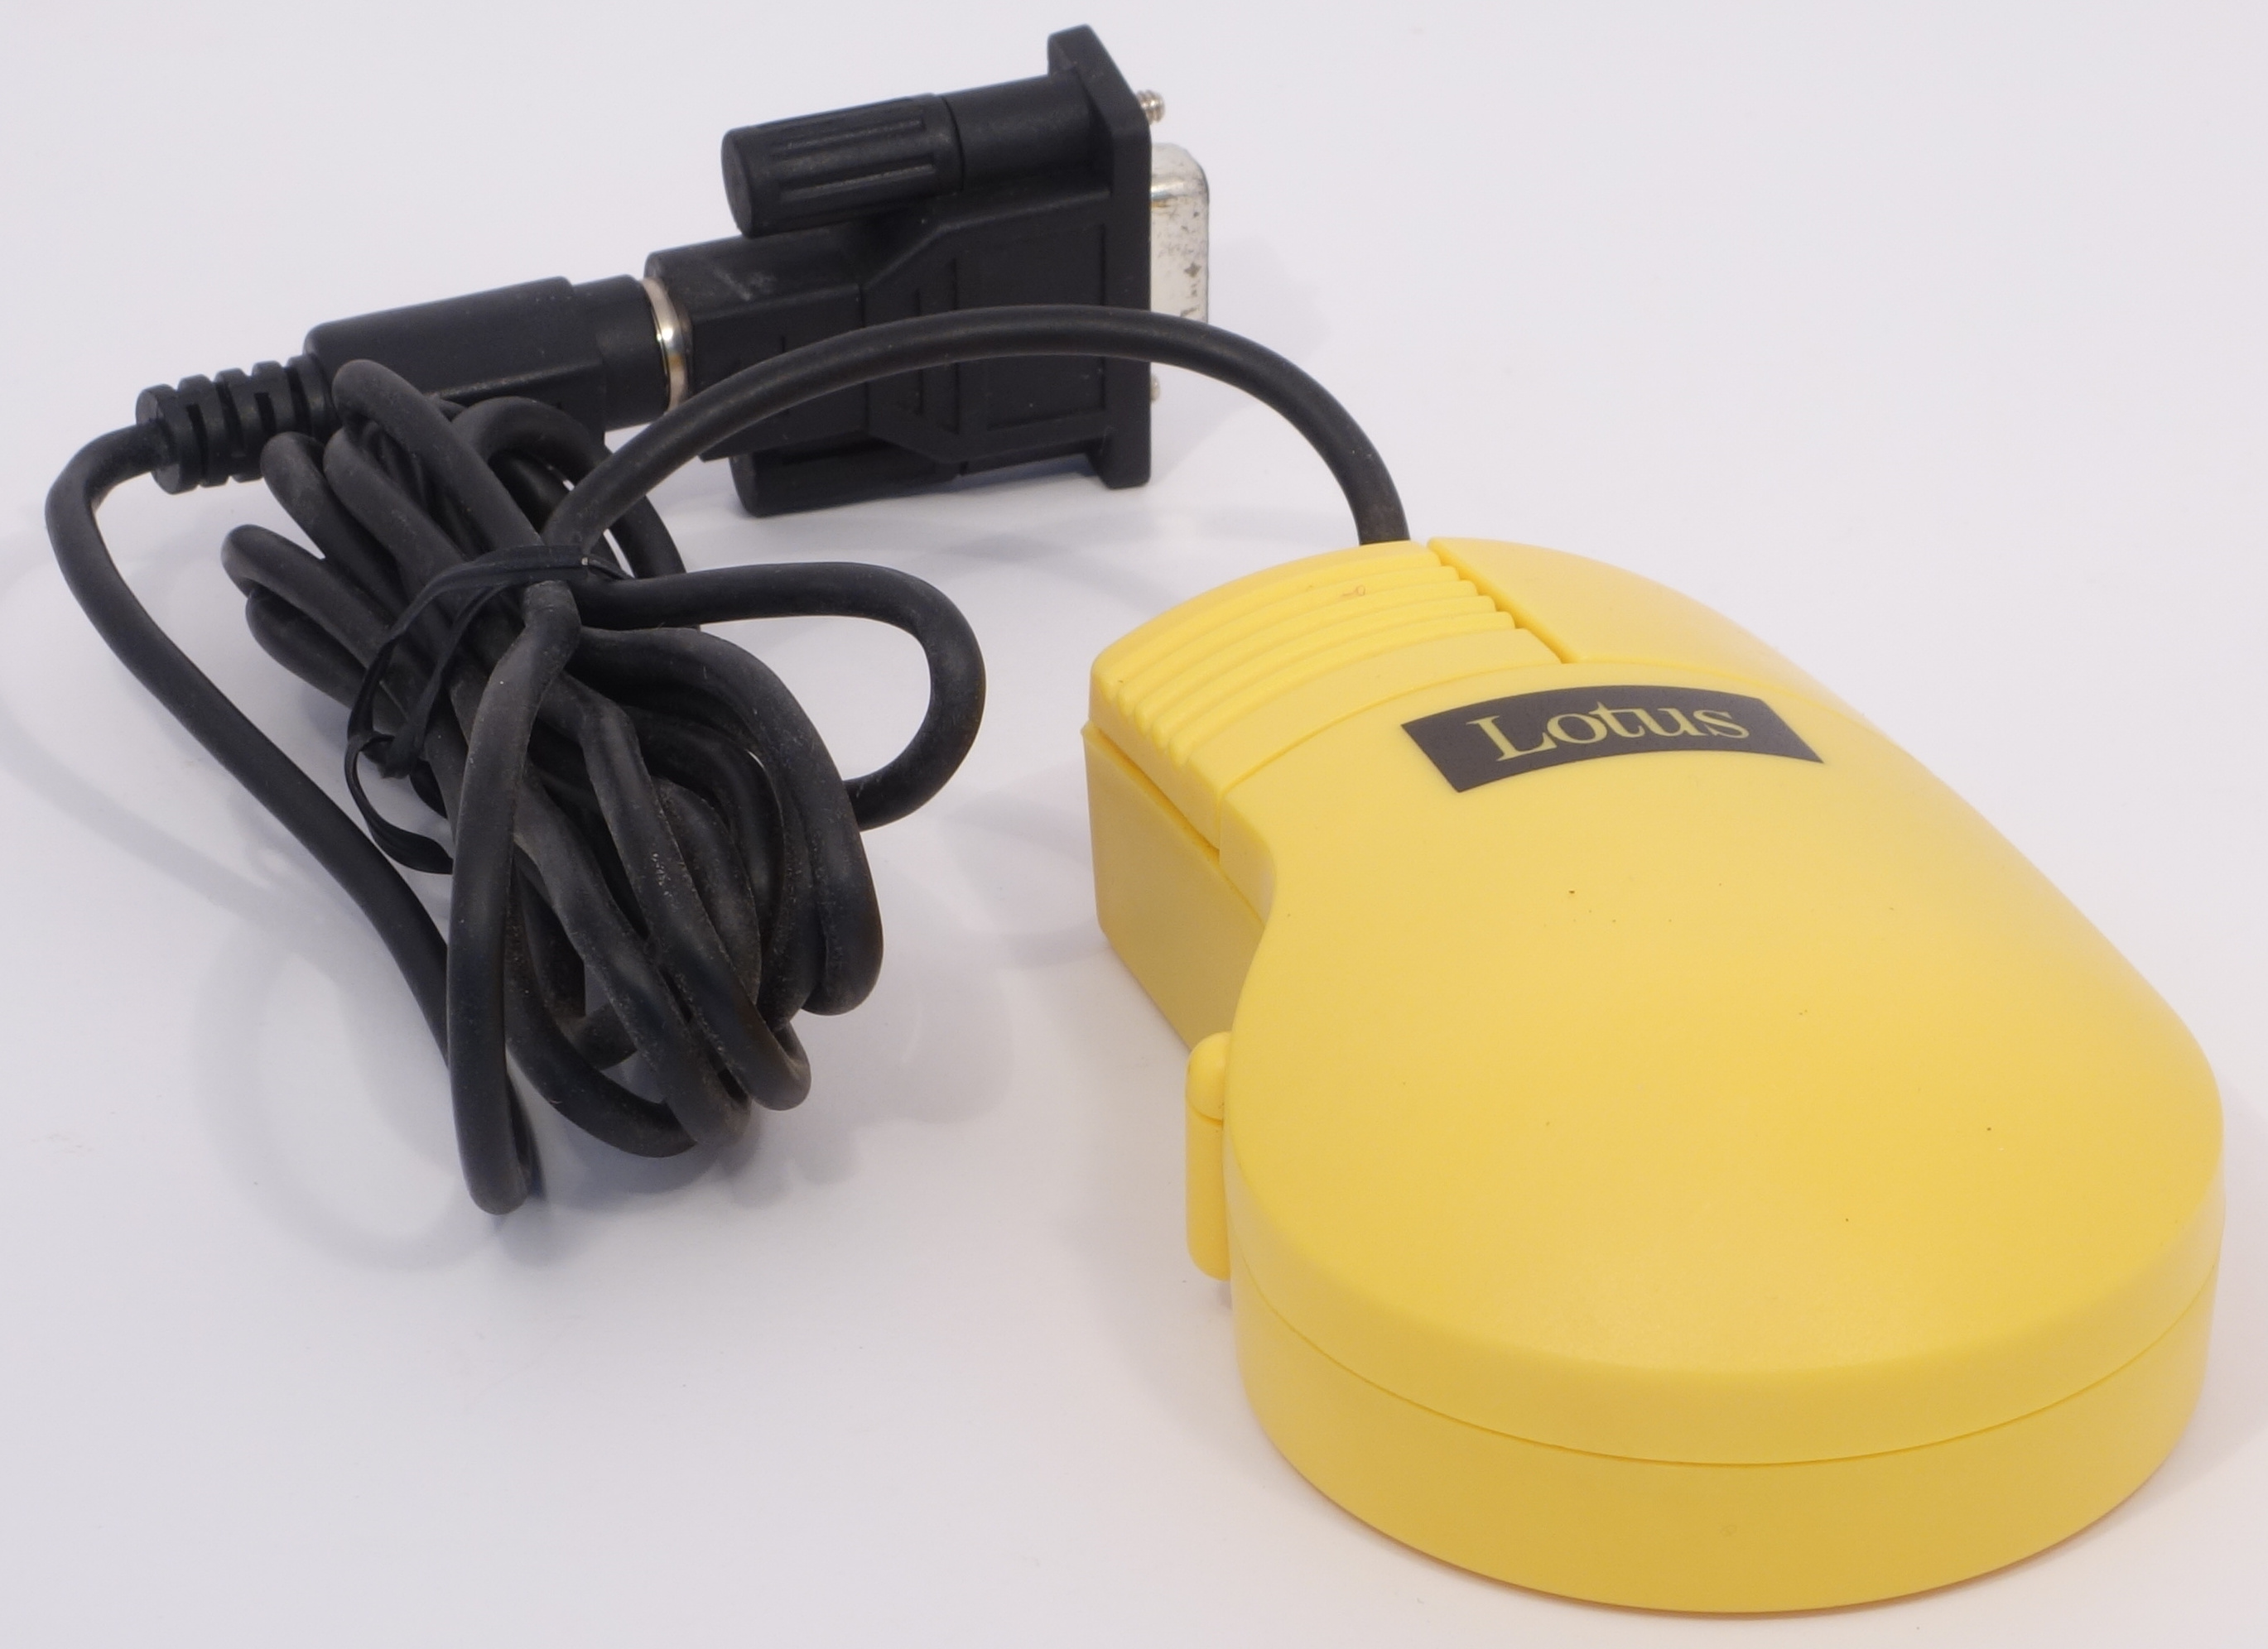
\includegraphics[scale=0.6]{1992_lotus_mouse/pic.jpg}
    \caption{Мышь Lotuse Mouse}
    \label{fig:LotusPic}
\end{figure}

Мышь имеет асимметричный корпус эргономичной формы и предназначена для использования правой рукой (рис. \ref{fig:LotusHand}). На верхней стороне корпуса присутствуют две кнопки большого размера и надпись Lotus. Поверхность главной кнопки мыши сделана рельефной, чтобы упростить ее тактильную идентификацию.

\begin{figure}[h]
    \centering
    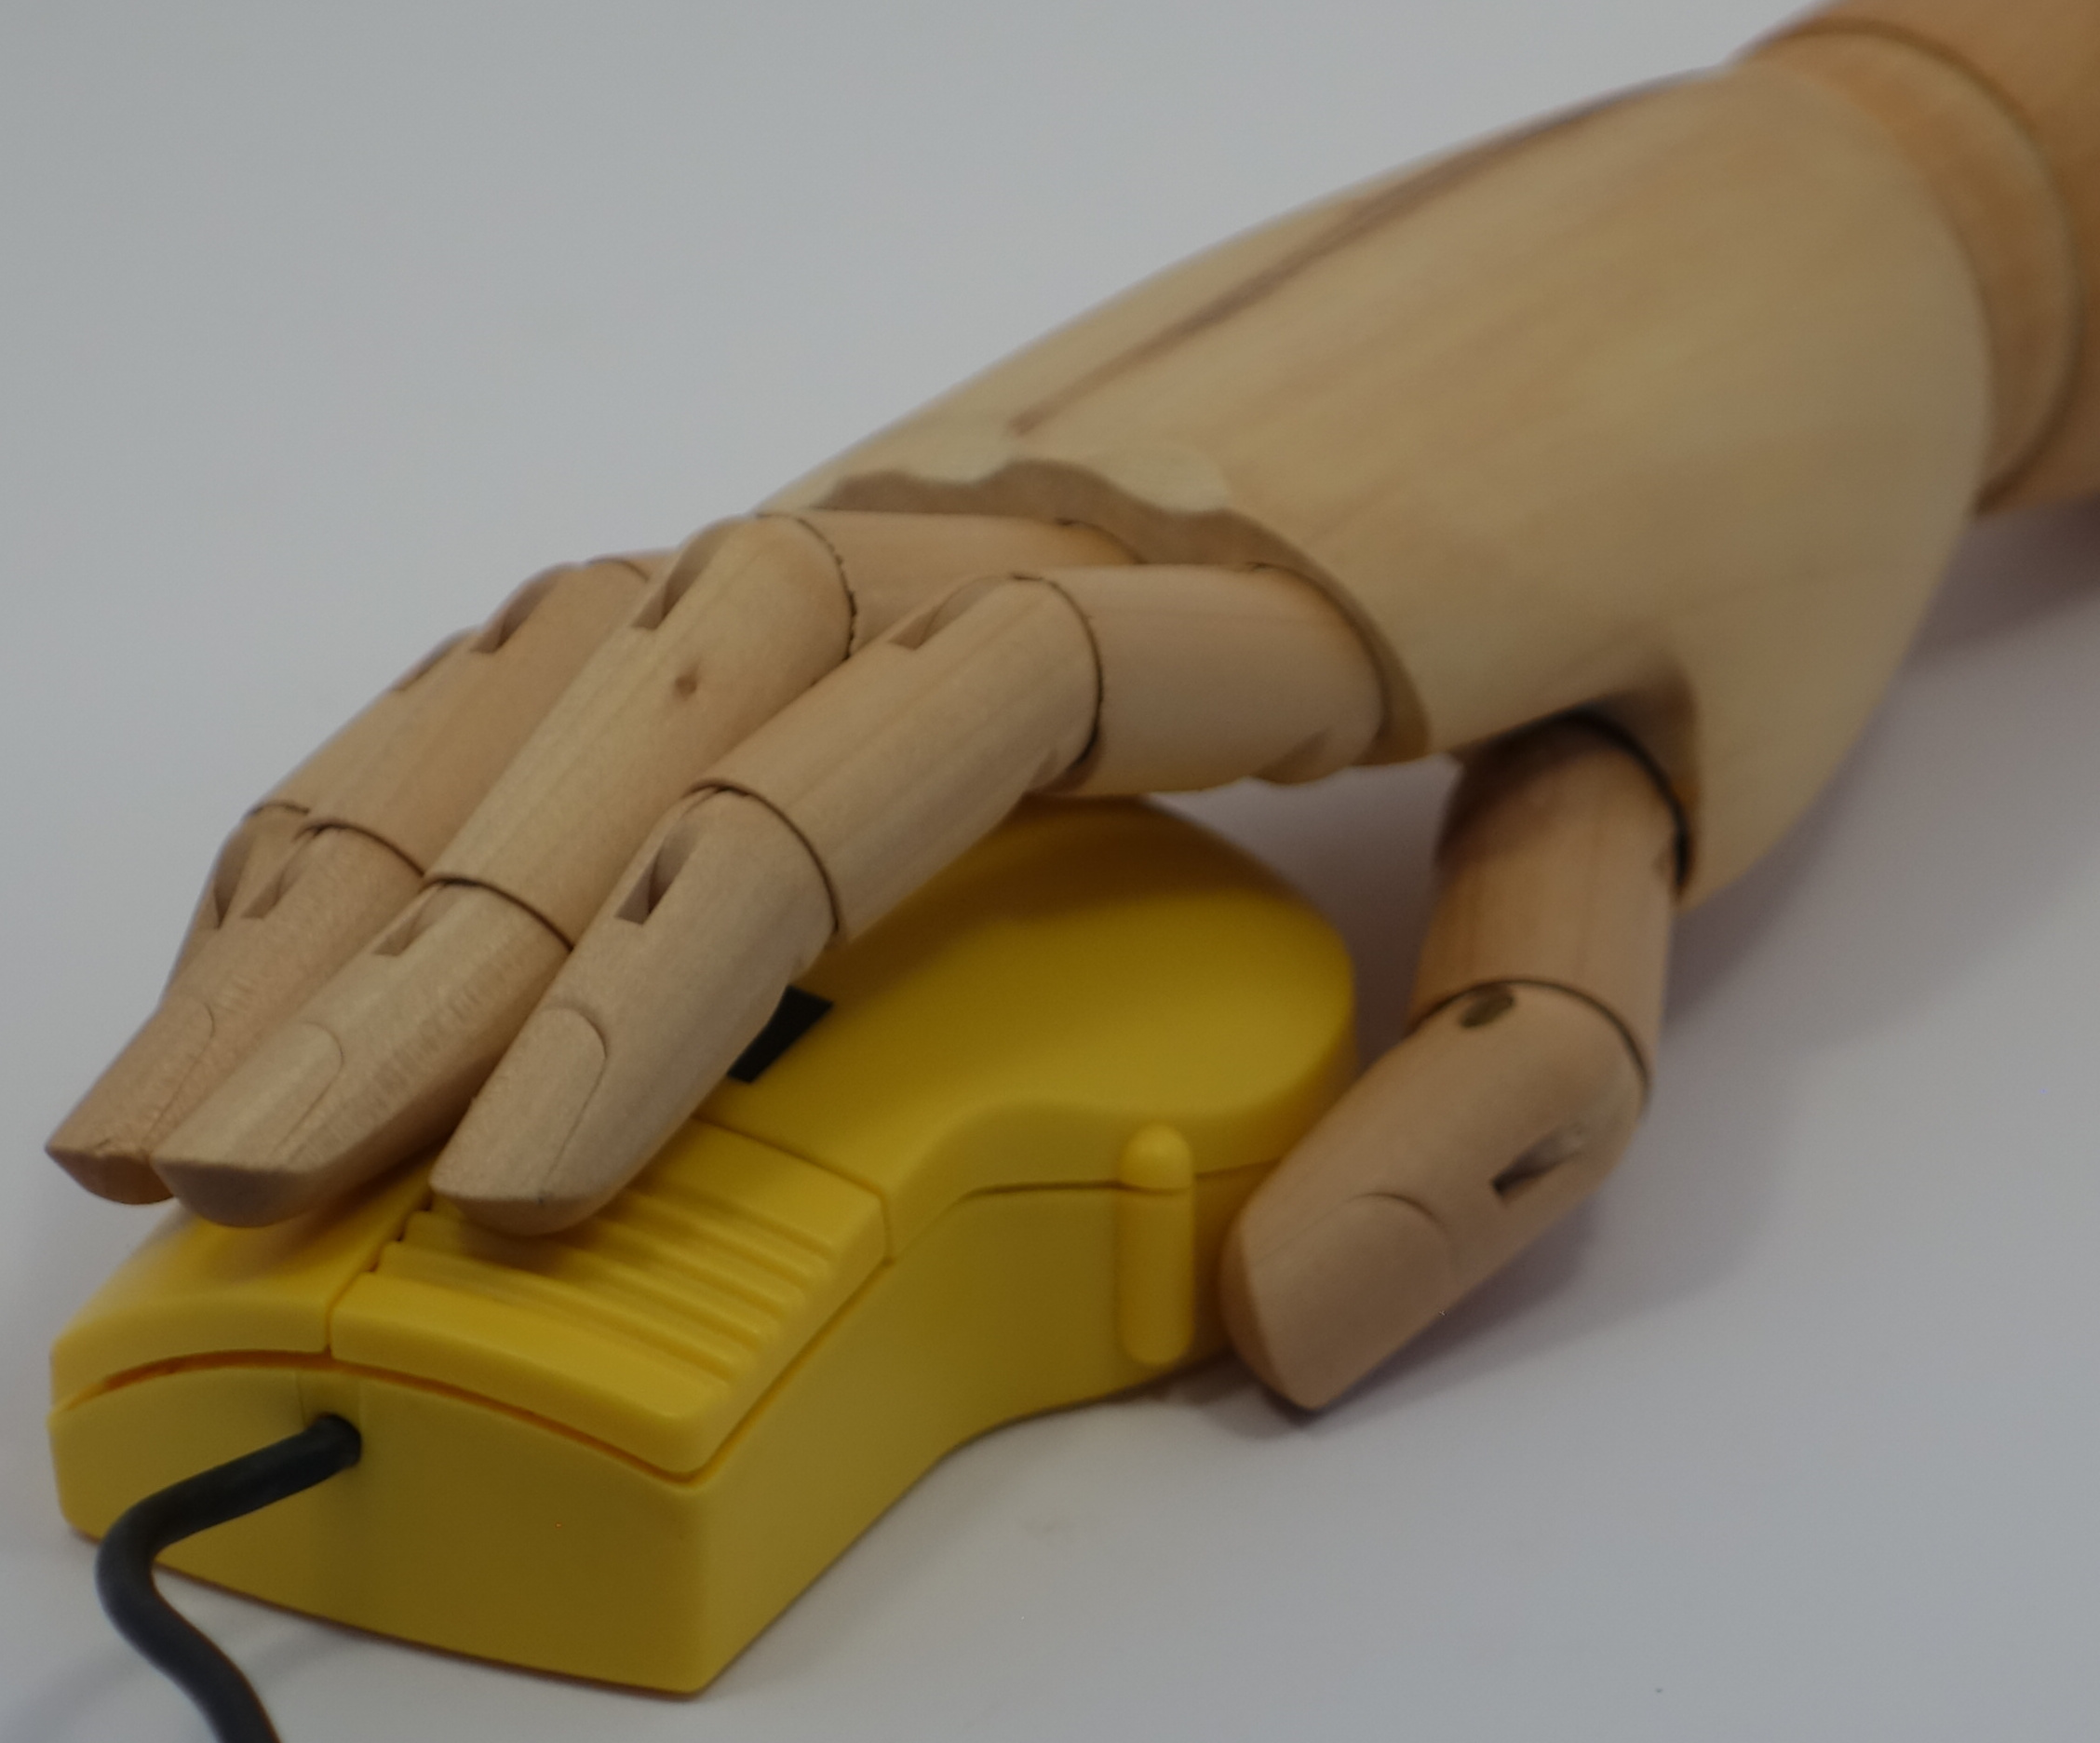
\includegraphics[scale=0.3]{1992_lotus_mouse/mis3.JPG}
    \caption{Изображение Lotuse Mouse с моделью руки человека}
    \label{fig:LotusHand}
\end{figure}

\begin{figure}[h]
    \centering
    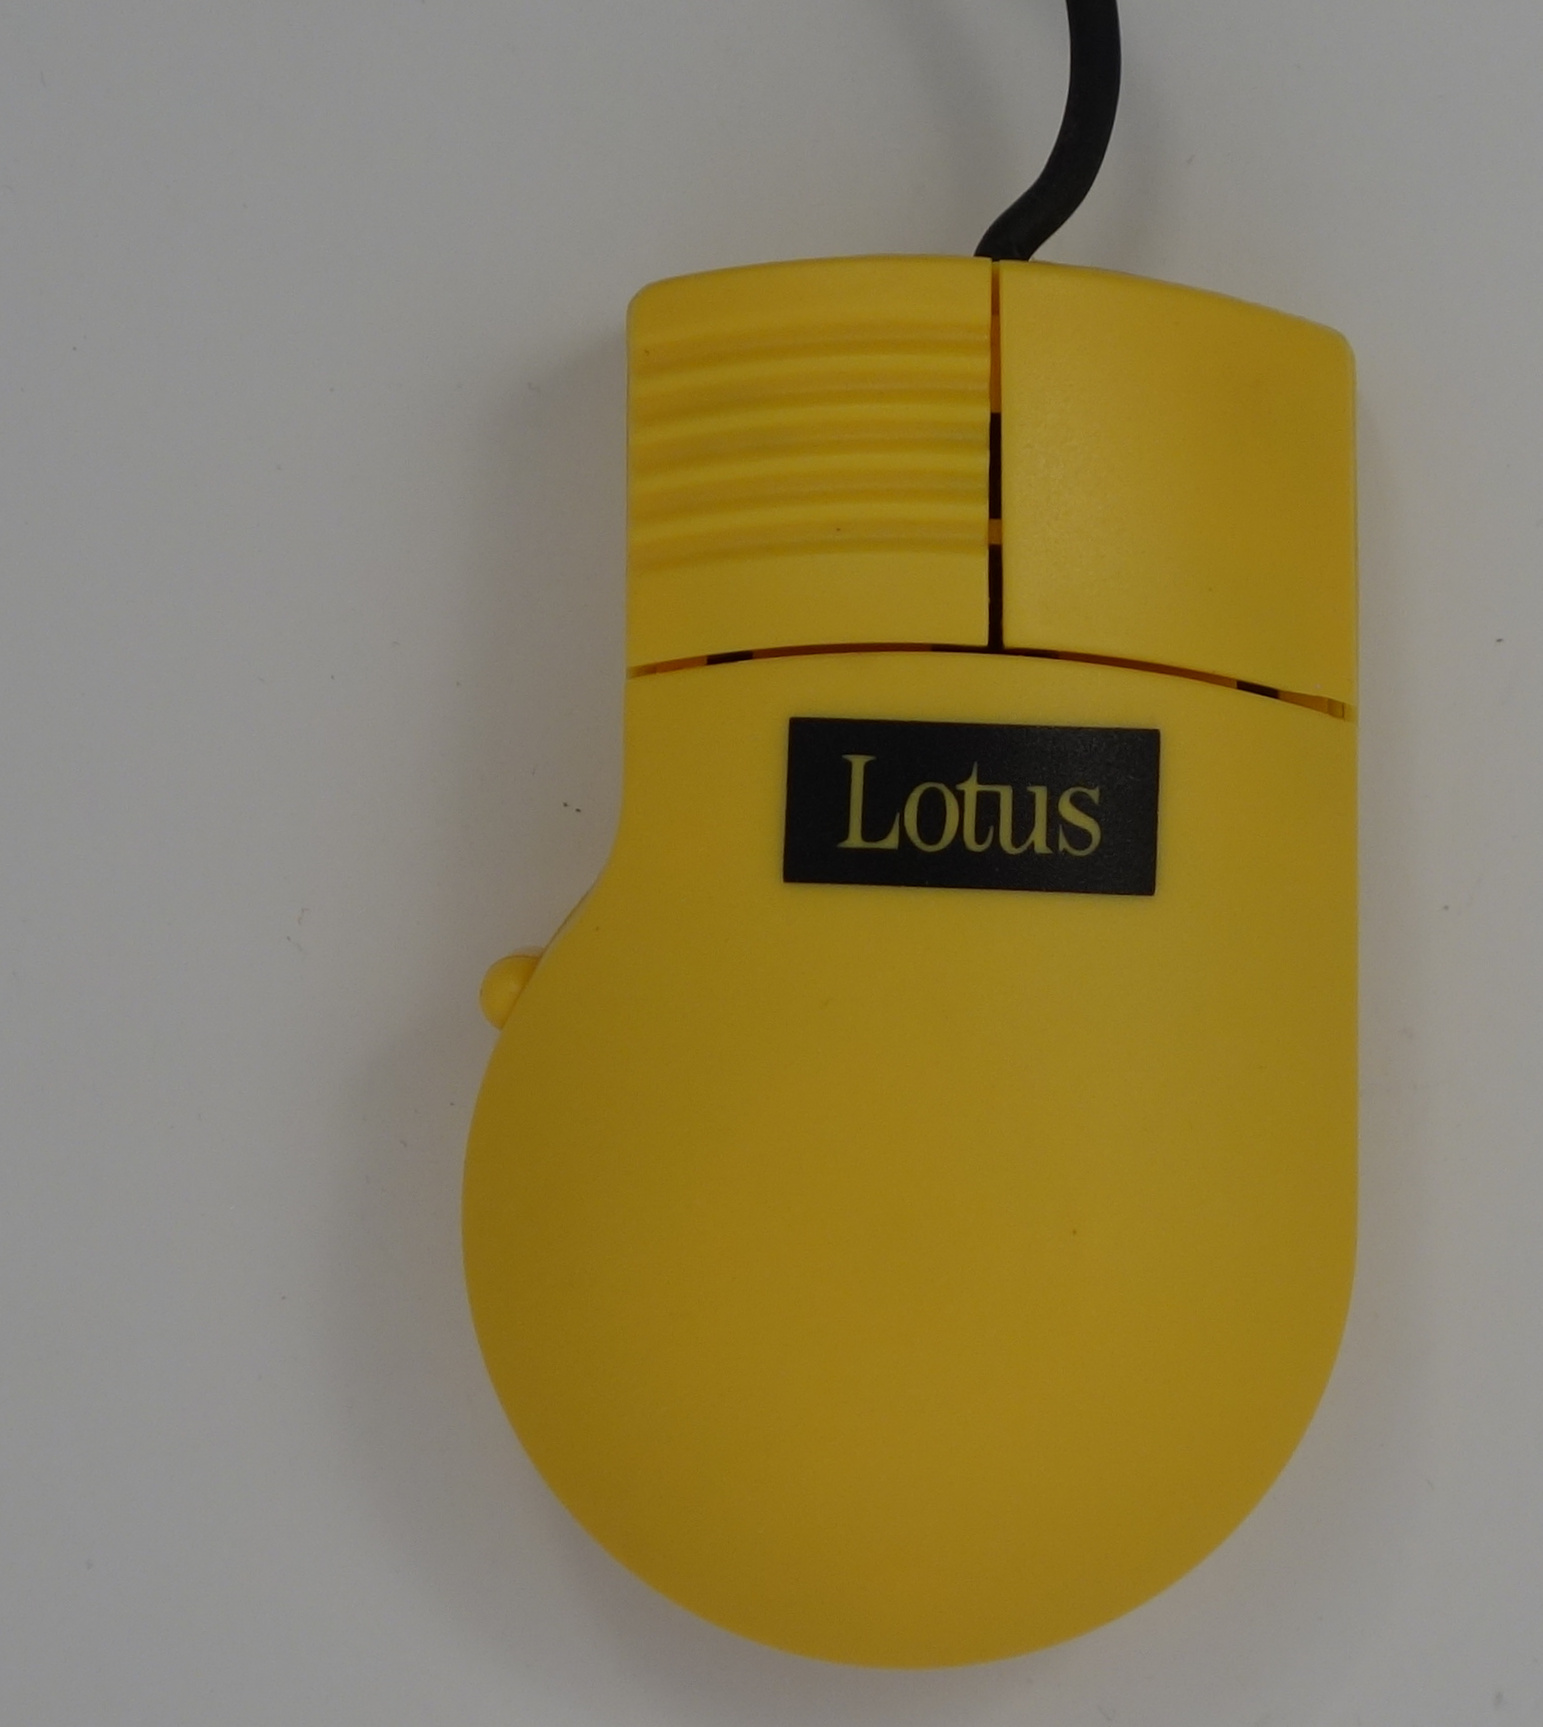
\includegraphics[scale=0.3]{1992_lotus_mouse/mis1.JPG}
    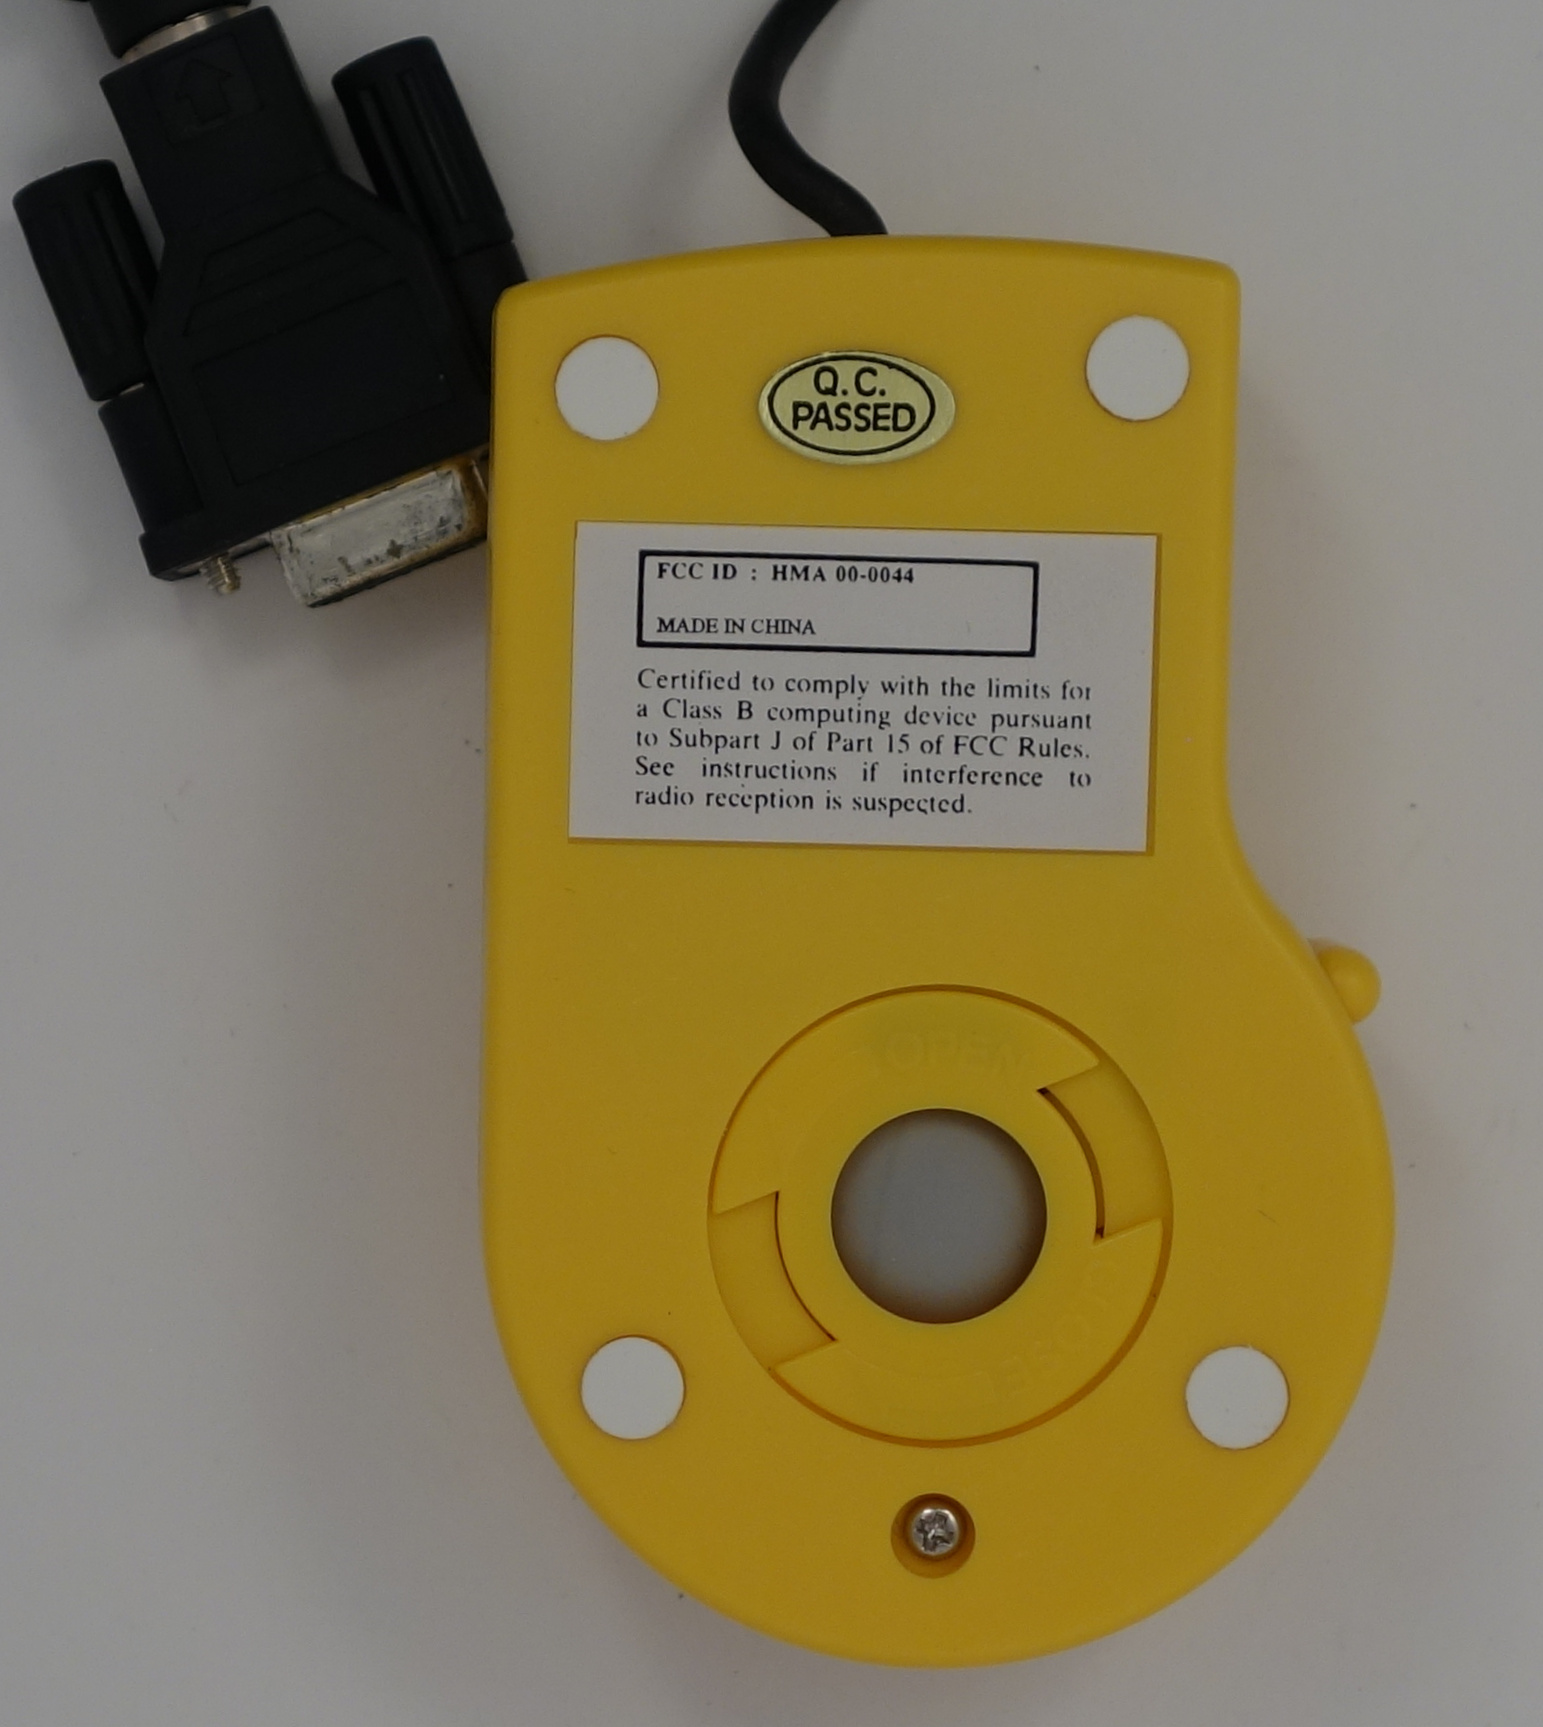
\includegraphics[scale=0.3]{1992_lotus_mouse/mis2.JPG}
    \caption{Lotuse Mouse, вид сверху и снизу}
    \label{fig:LotusTopBottom}
\end{figure}

Перевернув мышь (рис. \ref{fig:LotusTopBottom}), можно увидеть обрезиненный шарик, ножки для скольжения по поверхности, выполненные из низкофрикционного полимера, а также маркировку мыши.

Мышь подключается к компьютеру через последовательный порт.

\begin{figure}[h]
    \centering
    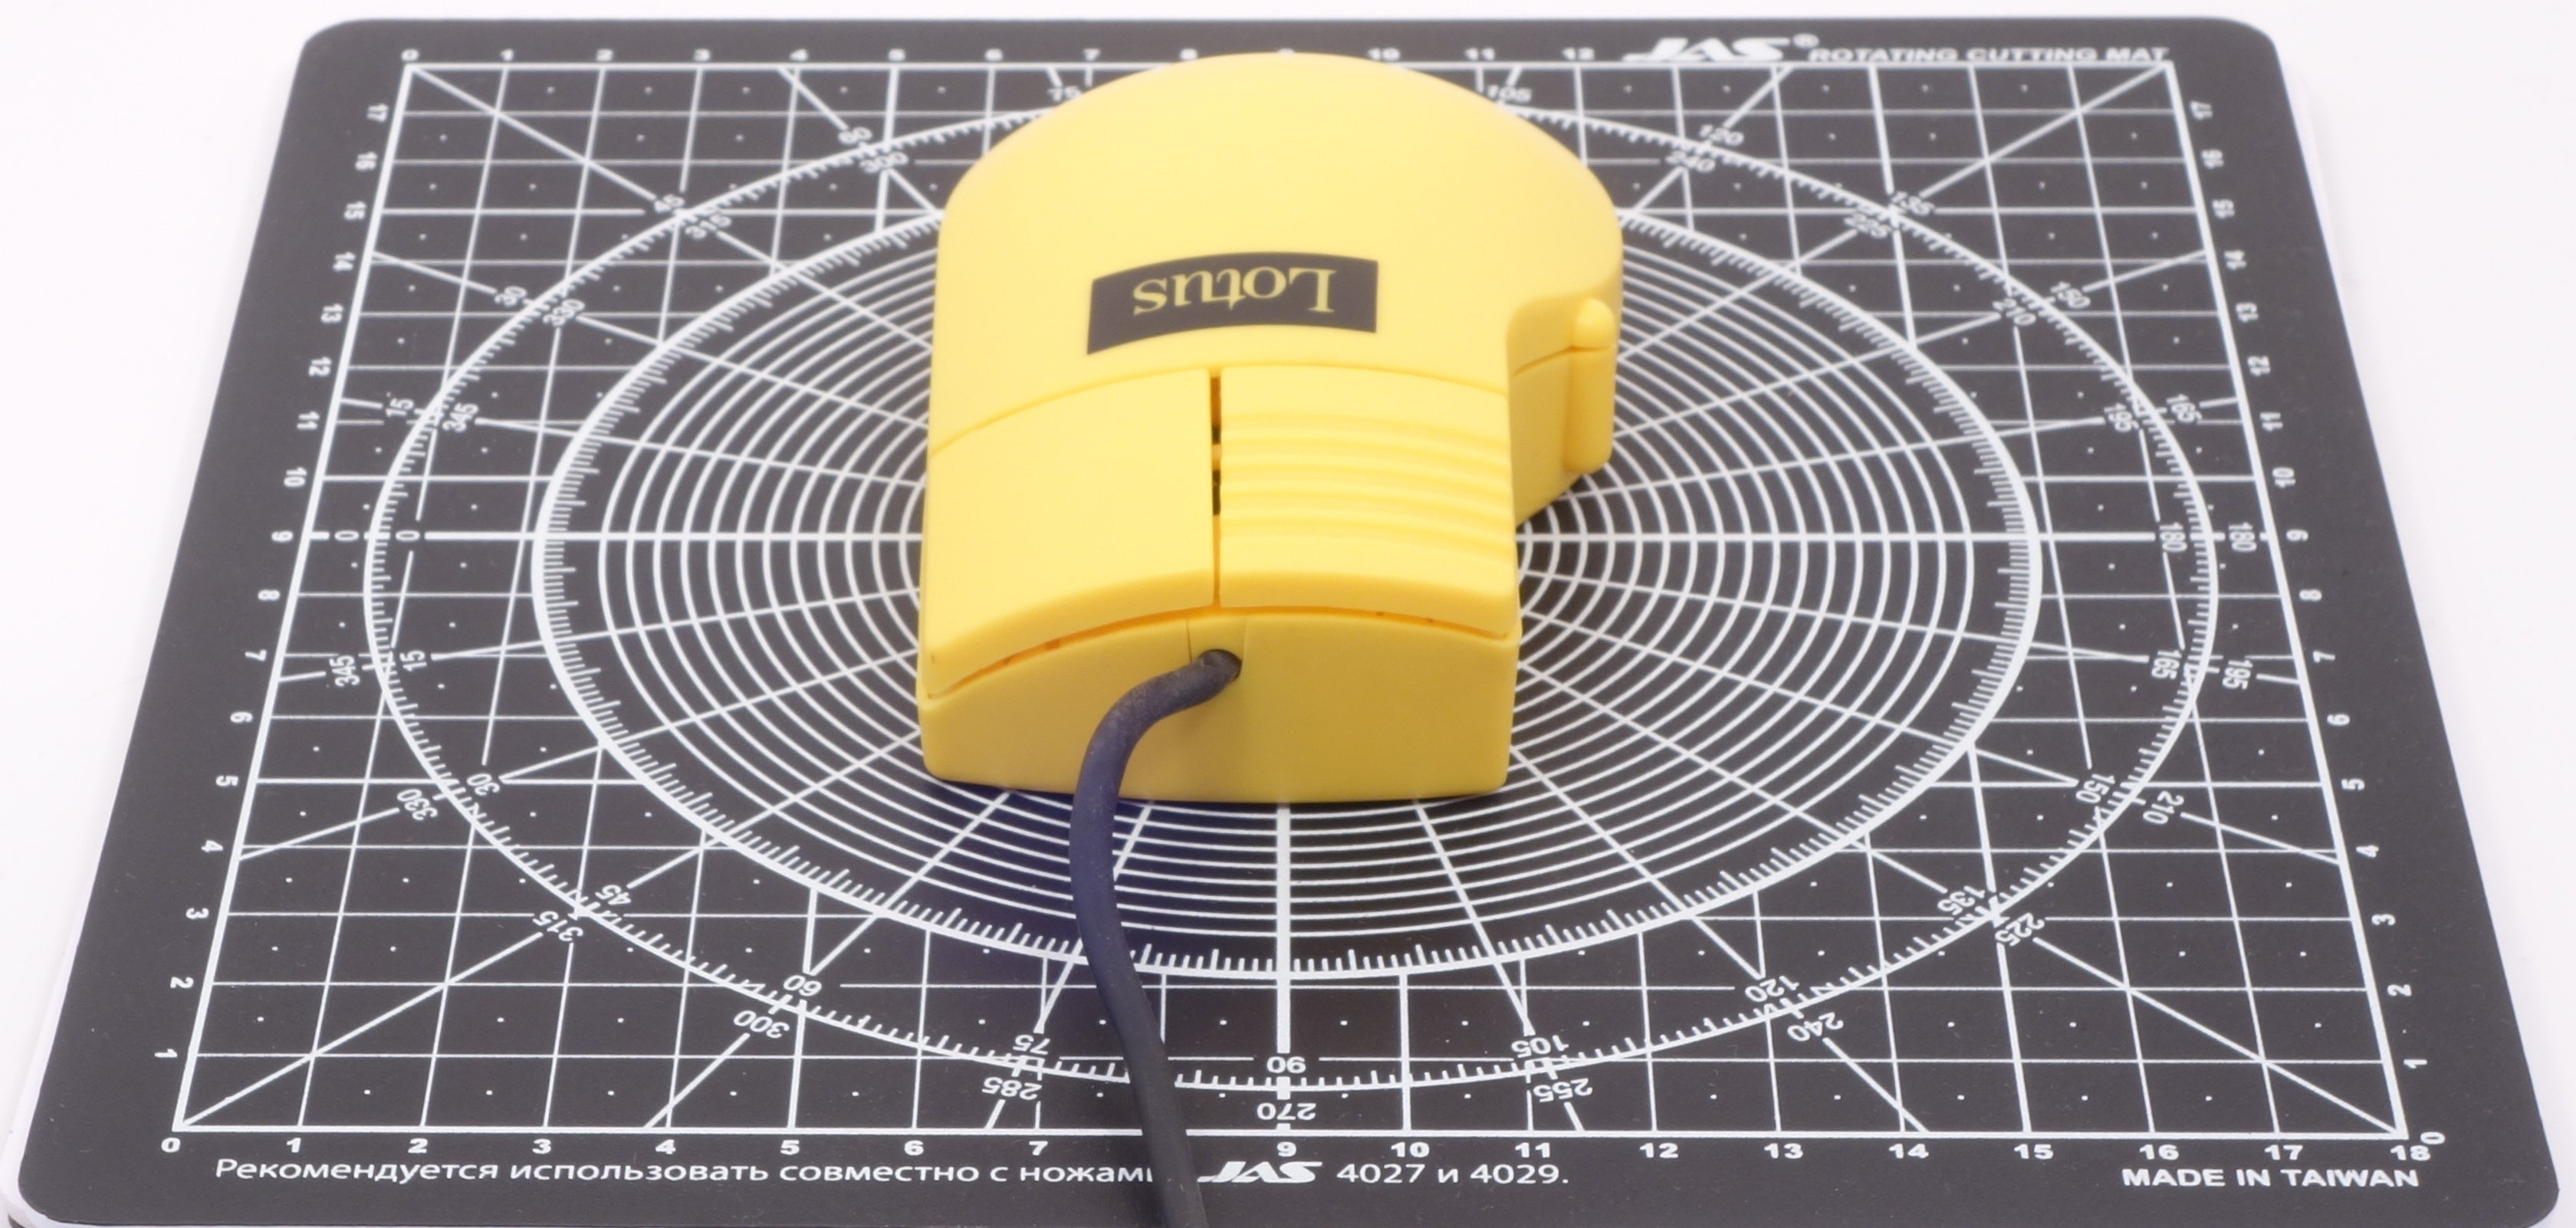
\includegraphics[scale=0.3]{1992_lotus_mouse/mis4.jpg}
    \caption{Изображение Lotuse Mouse на размерном коврике с шагом сетки 1~см}
    \label{fig:LotusSize}
\end{figure}

Можно сказать, что Lotus Mouse в определенной степени предвосхищает форму мыши Microsoft Mouse 2.0, которая была выпущена годом позже, а затем в свою очередь подарила форму самой известной мыши Microsoft "--- IntelliMouse.

\begin{figure}[h]
    \centering
    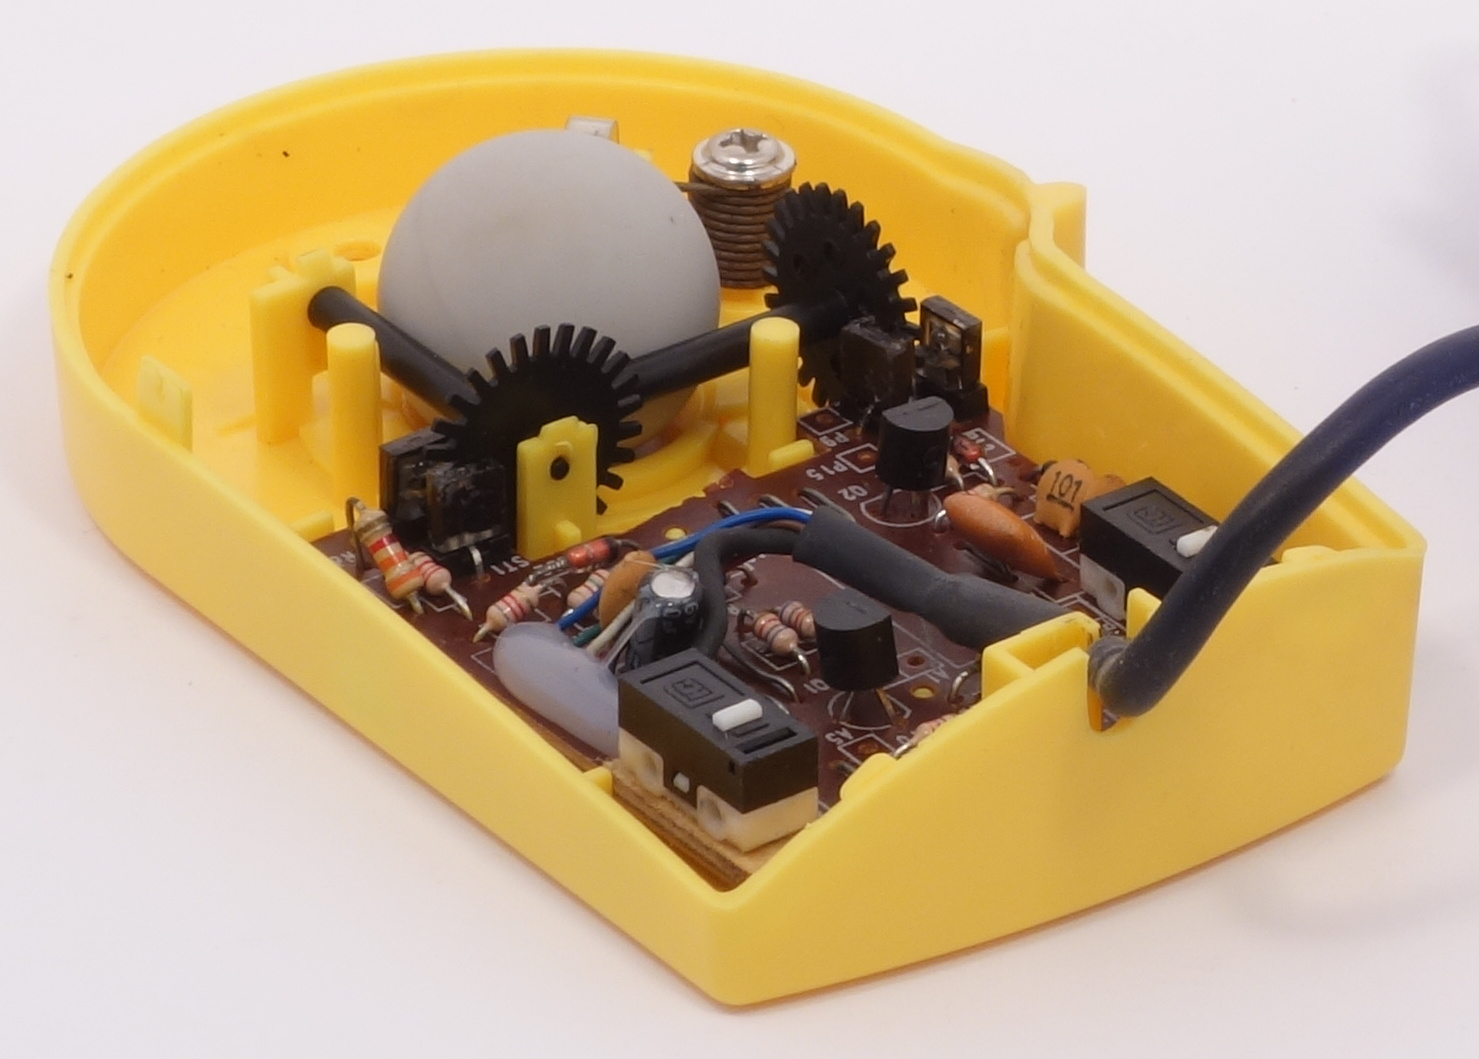
\includegraphics[scale=0.6]{1992_lotus_mouse/razob2.jpg}
    \caption{Lotuse Mouse в разобранном состоянии}
    \label{fig:LotusInside}
\end{figure}

Внутреннее устройство данного манипулятора показано на рис. \ref{fig:LotusInside}, что позволяет классифицировать его как традиционную оптомеханическую конструкцию. Изучение кода FCC ID по базе данных Федеральной комиссии по связи США показывает, что мышь была изготовлена в 1992 году на заводе в Сингапуре тайваньской компанией BMC Micro Industries.
\end{document}
